\documentclass[border=4pt,12pt]{standalone}
% House style for redrawn exam diagrams (diagram-v4: 0.4pt lines, filled -latex arrows, fine dashes; stipple and hatching drawn as real dots/lines (no PDF/SVG patterns, so they render in every browser and at any scale); transparent background). Every figure \input's this.
\usepackage{amsmath,amssymb}
\usepackage{txfonts}
\usepackage{pdfrender,xcolor}
% \halo{text}: label on shading. The shading stops just around each letter's outline (a thin knock-out that follows the
% glyphs, like the papers' typesetting), never a box. Owner: "I don't want a box around the text".
\newcommand{\halo}[1]{\leavevmode\rlap{\pdfrender{TextRenderingMode=2,LineWidth=2.2pt,LineJoinStyle=1,StrokeColor=white,FillColor=white}#1}#1}
\usepackage{tikz,pgfplots}
\pgfplotsset{compat=1.18}
\usetikzlibrary{arrows.meta,calc,angles,quotes,patterns,patterns.meta,intersections,positioning,decorations.markings,shapes.geometric}
% Stipple and hatching are drawn as actual dots / lines clipped to the region (path picture), NOT as pattern fills:
% SVG <pattern> fills vanish or blur when browsers scale the image, so the owner could not see the shading.
% Each dot is a 0.72pt square (keeps SVGs small; reads as a dot at print size). Dots sit on one global staggered grid, so neighbouring regions line up.
\makeatletter
\newdimen\ex@x \newdimen\ex@y \newdimen\ex@xa \newdimen\ex@ya \newdimen\ex@xb \newdimen\ex@yb \newcount\ex@row
\def\exam@stipplecolor{black!75}\def\exam@dotr{0.42pt}\def\exam@dotgap{2.5}
\def\ex@rowdots{\ifdim\ex@x<\ex@xb \pgfpathrectangle{\pgfqpoint{\dimexpr\ex@x-0.36pt\relax}{\dimexpr\ex@y-0.36pt\relax}}{\pgfqpoint{0.72pt}{0.72pt}}\advance\ex@x by \exam@dotgap pt\relax\expandafter\ex@rowdots\fi}
\def\exam@stipple{%
  \pgftransformreset% dots are sized in real points even inside scaled pictures
  \pgfpointanchor{path picture bounding box}{south west}\ex@xa=\pgf@x \ex@ya=\pgf@y
  \pgfpointanchor{path picture bounding box}{north east}\ex@xb=\pgf@x \ex@yb=\pgf@y
  \pgfsetfillcolor{\exam@stipplecolor}\pgfmathsetmacro\ex@h{\exam@dotgap/2}%
  \pgfmathtruncatemacro\ex@r{floor(\ex@ya/\ex@h)-1}\ex@row=\ex@r\relax
  \ex@y=\ex@r\dimexpr\ex@h pt\relax
  \loop\ifdim\ex@y<\ex@yb
    \pgfmathtruncatemacro\ex@c{floor(\ex@xa/\exam@dotgap)-1}\ex@x=\ex@c\dimexpr\exam@dotgap pt\relax
    \ifodd\ex@row \advance\ex@x by \ex@h pt\fi
    \ex@rowdots
    \advance\ex@y by \ex@h pt \advance\ex@row by 1
    \ifnum\numexpr\ex@row-(\ex@row/4)*4\relax=0 \pgfusepath{fill}\fi% flush every 4 rows: bounded TeX memory, few clip copies in the SVG
  \repeat\pgfusepath{fill}}
\newdimen\ex@d
\def\exam@hatch#1{% #1 = 1 for /, -1 for \ ; lines 45 degrees, 3pt apart
  \pgftransformreset
  \pgfpointanchor{path picture bounding box}{south west}\ex@xa=\pgf@x \ex@ya=\pgf@y
  \pgfpointanchor{path picture bounding box}{north east}\ex@xb=\pgf@x \ex@yb=\pgf@y
  \ex@d=\dimexpr\ex@yb-\ex@ya\relax \ex@x=\dimexpr\ex@xa-\ex@d\relax
  \loop\ifdim\ex@x<\ex@xb
    \ifnum#1>0 \pgfpathmoveto{\pgfqpoint{\ex@x}{\ex@ya}}\pgfpathlineto{\pgfqpoint{\dimexpr\ex@x+\ex@d\relax}{\ex@yb}}%
    \else \pgfpathmoveto{\pgfqpoint{\ex@x}{\ex@yb}}\pgfpathlineto{\pgfqpoint{\dimexpr\ex@x+\ex@d\relax}{\ex@ya}}\fi
    \advance\ex@x by 4.24pt
  \repeat
  \pgfsetlinewidth{0.4pt}\pgfsetstrokecolor{black}\pgfusepath{stroke}}
\def\examstipple{\exam@stipple}\def\examhatch{\exam@hatch}\def\examsetstipplecolor#1{\def\exam@stipplecolor{#1}}\def\examsetdotgap#1{\def\exam@dotgap{#1}}
\makeatother
% (legacy pattern kept for old files)
% staggered stipple like the NESA papers' dotted shading
\pgfdeclarepatternformonly{exam stipple}{\pgfpointorigin}{\pgfqpoint{2.2pt}{2.2pt}}{\pgfqpoint{2.2pt}{2.2pt}}{%
  \pgfpathcircle{\pgfqpoint{0.55pt}{0.55pt}}{0.42pt}\pgfpathcircle{\pgfqpoint{1.65pt}{1.65pt}}{0.42pt}\pgfusepath{fill}}
\tikzset{
  every picture/.style={line width=0.6pt, >={Latex[length=2mm,width=1.3mm]}},
  curve/.style={line width=0.6pt},
  open arrow/.style={-{Latex[length=2mm,width=1.3mm]}},  % owner: filled -latex heads everywhere, no open chevrons
  aux/.style={dash pattern=on 2pt off 1.5pt, line width=0.6pt},
  shade/.code={\def\exA{#1}\def\exB{none}\ifx\exA\exB\else\pgfkeysalso{fill=black!18}\fi},
  shade/.default=on,
  shade dots/.style={fill=none, path picture={\examstipple}},
  stipple color/.code={\examsetstipplecolor{#1}},
  stipple gap/.code={\examsetdotgap{#1}},
  shade dense dots/.style={fill=none, stipple gap=1.6, path picture={\examstipple}},
  shade hatch/.style={fill=none, path picture={\examhatch{1}}},
  shade hatch reverse/.style={fill=none, path picture={\examhatch{-1}}},
  shade solid/.style={fill=black},
  pt/.style={circle, fill, inner sep=1.1pt},
  open pt/.style={circle, draw, fill=white, inner sep=1.1pt},
}
\pgfplotsset{
  exam axes/.style={axis lines=middle, axis line style={->}, xlabel={$x$}, ylabel={$y$},
    xlabel style={anchor=west}, ylabel style={anchor=south}, tick label style={font=\small},
    every axis plot/.append style={line width=0.6pt, black}, samples=200, clip=false,
    enlargelimits=false, axis on top},
}

\begin{document}
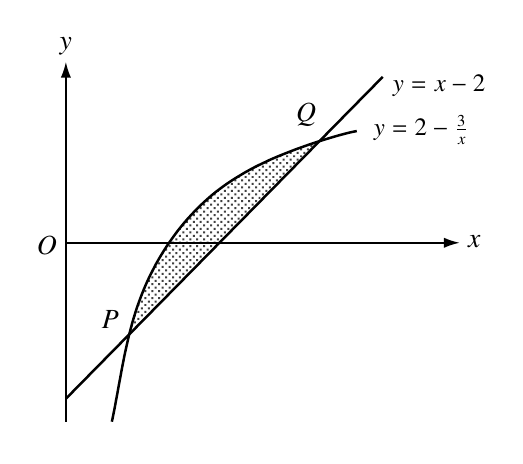
\begin{tikzpicture}[x=0.0127cm,y=-0.0127cm]
  \begin{scope}
    \clip (60,418) -- (450,22) -- (60,22) -- cycle;
    \fill[shade dots] plot[smooth] coordinates {(143,404) (144.5,396.8) (145.9,389.7) (147.2,382.5) (148.6,375.1) (149.9,367.8) (151.3,360.4) (152.6,353.2) (154,346) (155.4,338.8) (156.9,331.7) (158.5,324.7) (160.1,317.7) (161.9,310.8) (163.7,304.1) (165.7,297.4) (167.8,290.7) (170.1,284.2) (172.5,277.8) (175.1,271.3) (177.8,265) (180.7,258.8) (183.8,252.7) (187,246.5) (190.4,240.5) (193.9,234.7) (197.6,228.9) (201.5,223.2) (205.5,217.6) (209.6,212.1) (213.9,206.8) (218.3,201.6) (222.9,196.6) (227.6,191.6) (232.4,186.9) (237.4,182.3) (242.4,177.9) (247.7,173.6) (253,169.6) (258.6,165.6) (264.2,161.9) (270,158.3) (275.9,154.8) (282,151.4) (288.1,148.2) (294.4,145.2) (300.7,142.2) (307.1,139.4) (313.7,136.7) (320.3,134.1) (327,131.5) (333.7,129.1) (340.5,126.7) (347.4,124.4) (354.3,122.2) (361.2,120.1) (368,118.1) (374.6,116.3) (381.3,114.6) (388,113.2)} -- (520,113) -- (520,420) -- cycle;
  \end{scope}
  \draw[->] (97,404) -- (97,44);
  \draw[->] (97,225) -- (491,225);
  \draw[line width=0.9pt] (97,381) -- (414,59);
  \draw[line width=0.9pt] plot[smooth] coordinates {(143,404) (144.5,396.8) (145.9,389.7) (147.2,382.5) (148.6,375.1) (149.9,367.8) (151.3,360.4) (152.6,353.2) (154,346) (155.4,338.8) (156.9,331.7) (158.5,324.7) (160.1,317.7) (161.9,310.8) (163.7,304.1) (165.7,297.4) (167.8,290.7) (170.1,284.2) (172.5,277.8) (175.1,271.3) (177.8,265) (180.7,258.8) (183.8,252.7) (187,246.5) (190.4,240.5) (193.9,234.7) (197.6,228.9) (201.5,223.2) (205.5,217.6) (209.6,212.1) (213.9,206.8) (218.3,201.6) (222.9,196.6) (227.6,191.6) (232.4,186.9) (237.4,182.3) (242.4,177.9) (247.7,173.6) (253,169.6) (258.6,165.6) (264.2,161.9) (270,158.3) (275.9,154.8) (282,151.4) (288.1,148.2) (294.4,145.2) (300.7,142.2) (307.1,139.4) (313.7,136.7) (320.3,134.1) (327,131.5) (333.7,129.1) (340.5,126.7) (347.4,124.4) (354.3,122.2) (361.2,120.1) (368,118.1) (374.6,116.3) (381.3,114.6) (388,113.2)};
  \node at (97,28) {$y$};
  \node at (505,224) {$x$};
  \node at (78,228) {$O$};
  \node at (141,302) {$P$};
  \node at (337,97) {$Q$};
  \node[anchor=west,font=\small] at (414,68) {$y=x-2$};
  \node[anchor=west,font=\small] at (395,112) {$y=2-\frac{3}{x}$};
\end{tikzpicture}
\end{document}
